\section{Assigned Classes}
The assigned class is the following:
\begin{itemize}
\item \texttt{ModelDataFileReader.java}
\end{itemize}

\noindent
The class is located in the {\texttt{org.apache.ofbiz.datafile} package of the Apache OFBiz project.

\section{Functional Role of Classes}
\subsection{Apache OFBiz}
The class to be reviewed is part of the \textit{Apache OFBiz} open-source project.

\textit{Apcahe OFBiz} is an open-source ERP (Enterprise Resource Planning) and CRM (Customer Relationship Management) system that provides a suite of applications that are useful to integrate and automate most business processes of an enterprise (e.g. accounting, e-commerce, project management, order processing...).

The applications provided in the suite are meant to be loosely coupled and are built on a common architecture. Because of this and the project being open-source, they can be customized easily.

The \textit{Wikipedia} page on the project~\cite{wiki_ofbiz} gives some interesting information about the overall structure: \textit{OFBiz} is structured in three distinct layers, namely the \textbf{Presentation Layer}, the \textbf{Business Layer} and the \textbf{Data Layer}.

The \textbf{Presentation Layer} is responsible for managing the components which take care of the presentation for each of the applications provided in the suite.

\noindent
The \textbf{Business Layer} defines and manages the actual services to be provided to the users; it also manages the work-flows and simple methods involved in the logic of the applications in the suite, as well as the security issues behind them.

\noindent
The \textbf{Data Layer} manages the data access, storage and interface to the database for the applications of the project in a relational way. The assigned class plays a key role for this layer, since it allows the import and management of external data as defined by the user.

\subsection{OFBiz's DataFile Tools}
Of all the functions provided by \textit{Apache OFBiz}, the assigned class belongs to the one involved with data import and external data handling; this is provided by the DataFile Tool, which is specifically included in the \lword{\texttt{org.apache.ofbiz.datafile}} package of the project.

The documentation for the DataFile Tool, as provided on the official \textit{Apache OFBiz Project Open Wiki}~\cite{apachewiki} and in the official \textit{javadoc}~\cite{ofbiz_jdoc}, describes the tool as follows:

\begin{quotation}
\textit{"There is a data import tool in OFBiz called the DataFile tool. It uses XML files that describe flat file formats (including character delimited, fixed width, etc.) and parses the flat files based on those definitions. It uses a generic object to represent a row in the flat file. It includes features like a line type code for each line and can support hierarchical flat files (i.e. where parent/child relationships are implied by sub-records). An XSD is provided to describe how the data file definition XML file should look."}
\end{quotation}

The tool is based on the concept of \textbf{definition files}, XML files following the XSD structure mentioned in the quotation above that contain one or more \textbf{data file definitions} each; \textbf{data file definitions}, in turn, are a key concept that represent the structure of the flat data files. Finally, another relevant concept is that of \textbf{data files}, which are nothing more but fixed-width or character delimited text files containing all data properly formatted.

\subsection{The \texttt{ModelDataFileReader.java} class}
The role of the assigned class within the DataFile Tools is that of reading XML definition files and creating\texttt{ModelDataFileReader} objects that are used by other classes in the package to access the subsiding flat data files. These readers are specific to the URL of the XML definition file resource and hence only represent the portion of the database that is addressed by that XML structure.

The following example, taken from the \textit{Apache OFBiz Project Open Wiki}, gives an idea of the structure specification to be followed when taking advantage of the DataFile Tools:

\begin{figure}[H]
\begin{center}
		\centerline{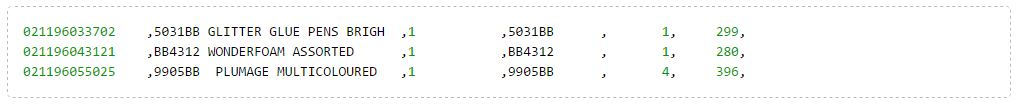
\includegraphics[width=1.3\textwidth]{./pictures/CSV_text_data_example.JPG}}
		\caption{An example of a fixed-width text file to be managed with the DataFile Tools.}
		\label{text_example}
\end{center}
\end{figure}

\begin{figure}[H]
\begin{center}
		\centerline{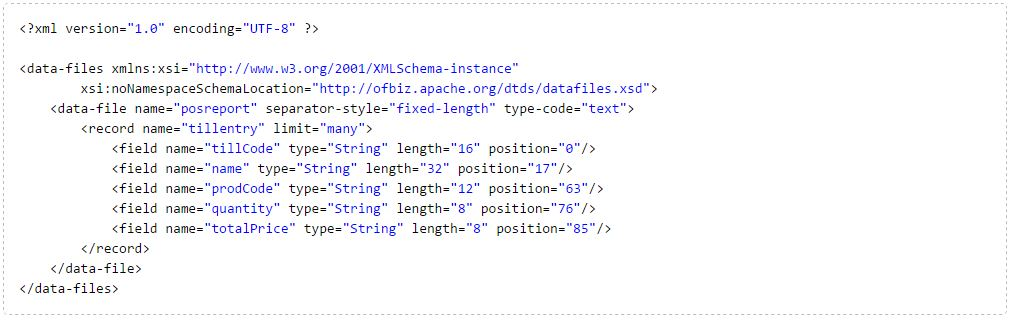
\includegraphics[width=1.3\textwidth]{./pictures/XML_structure_example.JPG}}
		\caption{An example of XML structure compliant with the XSD definition mentioned above.}
		\label{text_example}
\end{center}
\end{figure}

\texttt{ModelDataFileReader} objects are instantiated by classes that need access to the data files (e.g. \lword{\texttt{DataFile}}) via the \lword{\texttt{getModelDataFileReader(URL readerURL)}} static method which, depending on which readers are already instantiated, either returns a new reader or the reference to an existing one.

If a new reader has to be instantiated, the constructor method is called and the initialization of the actual \lword{\texttt{ModelDataFile}s} - which are the objects containing the structure for the data files - takes place. This happens through a call from the constructor to the \lword{\texttt{createModelDataFiles()}} method, which takes care of filling the {\texttt{modelDataFiles} map attribute of the reader with all the \lword{\texttt{ModelDataFile}} objects associated with it.

The above operation is an iterative procedure over the - possibly many - data file definitions that takes advantage, within its code, of the \lword{\texttt{createModelDataFile(Element dataFileElement)}} method, which is responsible for properly structuring and formatting the individual \lword{\texttt{ModelDataFile}} objects to be inserted in the \lword{\texttt{Map modelDataFiles}} attribute.

In turn, said procedure calls the \texttt{createModelRecord(Element recordElement)} method to perform a similar operation over the records (one or more) contained within a single \lword{\texttt{ModelDataFile}}; the same happens within said method, which calls the \lword{\texttt{createModelField(Element fieldElement)}} which creates the structure of single \lword{\texttt{ModelField}} objects.

A \lword{\texttt{ModelRecord}} is an object indicating the structure of the individual data blocks within the data files. A \lword{\texttt{ModelField}} is an object representing the structure of the individual data "tuples" contained in each record.

%%possibly explanation diagram?

The other methods of the class are interfacing methods, and provide a way for other classes to access the data structure encapsulated in the class by protecting the real data representation of textual files. In detail, there are:

\begin{itemize}
\item A \texttt{getDataFileNames()}, which returns a collection containing the names of the data files listed and described in the XML descriptor file;
\item A \texttt{getDataFileNamesIterator()}, which returns an iterator on the String names of the same data files;
\item A \lword{\texttt{getModelDataFile(String DataFileName)}}, which returns a single \texttt{ModelDataFile} based on its name in the XML descriptor file;
\item A \lword{\texttt{getModelDataFiles()}}, which returns the map containing all the \texttt{ModelDataFile}s accessible by the reader.
\end{itemize}

It is interesting to note that the assigned class is marked as \lword{\texttt{final}}, and hence can not be extended by other classes. This was done, most probably, as a design choice: the class was not designed for being extendible because the functionalities it provides must not be changed or, in fact, extended by other readers.